\documentclass{article}

\usepackage[utf8]{inputenc}
\usepackage[T1]{fontenc}
\usepackage{amssymb}
\usepackage{ntheorem}
\usepackage{amsmath}
\usepackage{multicol}
\usepackage{amssymb}
\usepackage[ a4paper, hmargin={3cm, 3cm}, vmargin={3cm, 3cm}]{geometry}

\usepackage{tikz}
\usetikzlibrary{automata,positioning}

\usepackage{tcolorbox}
\tcbuselibrary{
  theorems,
  breakable,
  skins
}

\usepackage{hyperref}
\hypersetup{
    colorlinks,
    citecolor=black,
    filecolor=black,
    linkcolor=blue,
    urlcolor=blue
}

\newtcbtheorem[number within=section]
{correction}{Correction}{
  colback=white,
  colframe=black!70,
  separator sign none,
  description delimiters parenthesis,
  enhanced jigsaw,
  breakable,
  fonttitle=\bfseries
}{}

\theoremstyle{plain}
\theorembodyfont{\normalfont}
\theoremseparator{~--}
\newtheorem{exercice}{Exercise}[section]

\newcommand{\dd}{\textit{dd}}

\title{TD n$^\circ$1}
\author{Valeran MAYTIE}
\date{}

\begin{document}
  \maketitle

  \section{Automata}

  \exercice Let $\mathcal A$ an automata, give an automata $\mathcal A_*$ such
    that $(L_{\mathcal A})^* = L_{\mathcal A_*}$

  \begin{correction}{}{}
    Let $\mathcal A = (Q, \Sigma, \delta, I, F)$, we want to construct $\mathcal
    A_*$:

    \begin{itemize}
      \item We add all initial states to the finite states for recognizing
        the empty word.

      \item And we define $\delta'$
      \[
        \delta' = \left \{
          \begin{tabular}{l l l r}
            $q, a$ & $\to$ & $\delta(q, a)$ &
              $a \in \Sigma, q \in Q$ \\
            $f, \varepsilon$ & $\to$ & $I$ & $\forall f \in F$\\
          \end{tabular}
          \right.
      \]
    \end{itemize}

    So at the end we have $\mathcal A_* = (Q, \Sigma, \delta', I, F \cup I)$
  \end{correction}

  \exercice Show that $(a|b)^* = (a^*b^*)^*$

  \begin{correction}{}{}
    We will proceed by double inclusion :

    \begin{itemize}
      \item[$\subseteq$ :] we will proof this inclusion by induction on the
        length of $w \in (a|b)^*$.
        \begin{itemize}
          \item If $|w| = 0$, so $w = \varepsilon \in (a^*b^*)^*$
          \item By induction hypothesis we know that all words $w$ of the length
            $n$ is in $(a^*b^*)^*$. We have two case for the words of length $n
            + 1$ :
          \begin{itemize}
            \item $w \cdot a$, $a \in (a|b)$ so by induction hypothesis we have
              $w\cdot a \in (a|b)^*(a|b) = (a|b)^*$.
            \item $w \cdot b$ same.
          \end{itemize}

        \end{itemize}
      \item[$\supseteq$ :] We know that $(a|b)^* = \Sigma^*$ so all words $w \in
        (a^*b^*)^*$ is on $(a|b)^*$ because $w \in \Sigma^*$
    \end{itemize}
  \end{correction}

  \exercice Give a DFA on $\Sigma = \{a, b\}$ recognizing all words having no
  more than two consecutive occurrences of the same letter.

  \begin{correction}{}{}
    \begin{center}
    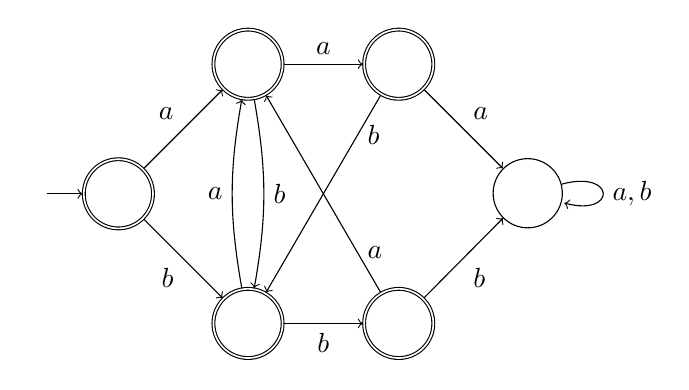
\begin{tikzpicture}[initial text=]
      \node[state, initial, accepting] (E) at (0, 0) { };
      \node[state, accepting] (A1) [above right= of E]  { };
      \node[state, accepting] (A2) [right= of A1]       { };
      \node[state, accepting] (B1) [below right= of E]  { };
      \node[state, accepting] (B2) [right= of B1]       { };
      \node[state]            (G)  [below right= of A2] { };

      \path[->] (E)  edge                 node[above left ] {$a$}    (A1)
                (A1) edge                 node[above      ] {$a$}    (A2)
                (A2) edge                 node[above right] {$a$}    (G)
                (E)  edge                 node[below left ] {$b$}    (B1)
                (B1) edge                 node[below      ] {$b$}    (B2)
                (B2) edge                 node[below right] {$b$}    (G)
                (G)  edge [loop right]    node[      right] {$a, b$} (G)
                (A1) edge [bend left=10]  node[      right] {$b$}    (B1)
                (B1) edge [bend left=10]  node[      left ] {$a$}    (A1)
                (B2) edge                 node[pos=0.2,right] {$a$}    (A1)
                (A2) edge                 node[pos=0.2,right] {$b$}    (B1)
      ;
    \end{tikzpicture}
    \end{center}
  \end{correction}

  \exercice
  We define the duplication of a word by : $\dd(\varepsilon) =
  \varepsilon$ and $\forall x \in \Sigma : \dd(v\cdots x) = \dd(v) \cdots xx$.
  \\
  Example : on $\Sigma = \{a, b\}$, $\dd(aba) = aabbaa$. We suppose that $L$ is
  a rational language. \\
  Show that $\dd(L) = \{\dd(v) | v \in L\}$ is rational to.

  \begin{correction}{}{}
    Let $\mathcal A_L =\{Q, \Sigma, \delta, I, F\}$ an automaton who recognize
    $L$.

    We construct $\mathcal A_{\dd(L)} = \{Q', \Sigma, \delta', I, F'\}$
    the automaton who recognize $\dd(L)$ :

    \begin{itemize}
      \item $Q' = Q \uplus Q = \{(i, q) | q \in Q, i \in \{0, 1\}\}$
      \item $F' = \{(q, 1) | q \in F\} \cup \{(q, 0),| q \in I \cap F\}$
      \item
        \[
        \delta' = \left \{
          \begin{tabular}{l l l r}
            $(q, 1), c$ & $\to$ & $\delta(q, c)$ & $c \in \Sigma$ \\
            $(q, 0), c$ & $\to$ & $(q, 1)$ & $c \in \Sigma$
          \end{tabular}
          \right.
      \]
    \end{itemize}
  \end{correction}

  \exercice Given an automaton $\mathcal A$, give a (non-deterministic)
  automaton recognizing $L^R$ the mirror language of $L_{\mathcal A}$.

  \begin{correction}{}{}
    Let $\mathcal A = \{Q, \Sigma, \delta, I, F\}$ an automaton who recognize
    $L$. So we have $\{Q, \Sigma, \delta', F, I\}$ with :
    $$\delta'(q, x) = \{q' | q \in \delta(q', x)\}$$
    an automaton who recognize $L^R$.
  \end{correction}

  \exercice Let $\Sigma = \{0, 1\}$ an alphabet.

    \begin{itemize}
      \item We consider a language $L_2$ the set of binary words representing a
        multiple of two. This language is recognizable ?

      \item Same question for $L_3$ the set of binary words representing a
        multiple of three.

      \item What about the $L_6$ language for binary words representing a
        multiple of 6 ?
    \end{itemize}

  \begin{correction}{}{}
    \begin{itemize}
      \item For $L_2$ we just need to recognize the words which end in 0 :

        \begin{center}
        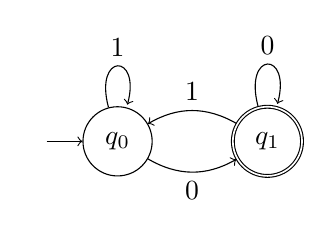
\begin{tikzpicture}[initial text=]
          \node[state, initial](q0) at (0,0) {$q_0$};
          \node[state, accepting] (q1) [right= of q0] {$q_1$};
          \path[->] (q0) edge[loop above] node[above] {1} (q0)
                    (q1) edge[loop above] node[above] {0} (q1)
                    (q0) edge[bend right] node[below] {0} (q1)
                    (q1) edge[bend right] node[above] {1} (q0);
        \end{tikzpicture}
        \end{center}

      \item For $L_3$ we have 3 $(n\bmod 3 \in \{0, 1, 2\})$.

        For each edge ($k$ the number read) :
        \begin{itemize}
          \item If we read a zero, new result : $2k$
          \item If we read a zero, new result : $2k + 1$
        \end{itemize}
        \begin{multicols}{2}
        \begin{tabular}{c | c | l}
          state & read & next \\
          \hline
          $q_0$ & 0    & $0 \times 2     \bmod 3 = 0$ \\
                & 1    & $0 \times 2 + 1 \bmod 3 = 1$ \\
                \hline
          $q_1$ & 0    & $1 \times 2     \bmod 3 = 2$ \\
                & 1    & $1 \times 2 + 1 \bmod 3 = 0$ \\
                \hline
          $q_2$ & 0    & $2 \times 2     \bmod 3 = 1$ \\
                & 1    & $2 \times 2 + 1 \bmod 3 = 2$ \\
        \end{tabular}
        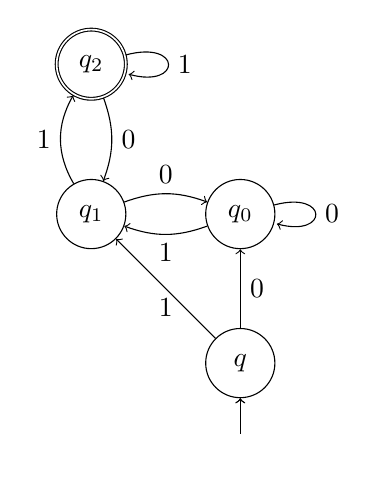
\begin{tikzpicture}[initial text=]
          \node[state]            (q1) at (0,0)            {$q_1$};
          \node[state, accepting] (q2) [above=of q1] {$q_2$};
          \node[state]            (q0) [right=of q1] {$q_0$};
          \node[state, initial, initial below] (q) [below=of q0] {$q$};

          \path[->] (q)  edge               node[below] {1} (q1)
                    (q)  edge               node[right] {0} (q0)
                    (q0) edge[bend left=20] node[below] {1} (q1)
                    (q0) edge[loop right]   node[right] {0} (q0)
                    (q1) edge[bend left]    node[left ] {1} (q2)
                    (q1) edge[bend left=20] node[above] {0} (q0)
                    (q2) edge[bend left=20] node[right] {0} (q1)
                    (q2) edge[loop right]   node[right] {1} (q2);
        \end{tikzpicture}
        \end{multicols}


      \item For $L_6$, we can use the same construction (7 states).

    \end{itemize}
  \end{correction}


  \exercice A Dyck language is the set $D$ of well-parenthesized words on an
  alphabet $\{\texttt (, \texttt )\}$. For example, the word
  \texttt{(()())(()(()))} is well parenthesized.

  This property can be formally defined :
  \begin{itemize}
    \item For any prefix $u$ of $w$, the number of $)$ in $u$ is less than the
      number of $($
    \item There are as many $($ as there are $)$ in the word
  \end{itemize}
  Show that $D$ is not a regular language.

  \begin{correction}{}{}
    Assume that $D$ is regular.

    We have the word $w = \texttt{(}^p \texttt{)}^p$ with $p \leq 1$.
    We pose $x = \varepsilon$, $y = \texttt(^p$ and $z = \texttt )^p$.

    The conditions are well verified : $|xy| \leq p$ and $|y| \geq 1$.

    If we consider the word $xy^2z$. This word has $2p$ \texttt ( and
    $p$ \texttt ). So $xy^2z$ is not in $D$.

    By the pumping lemma $D$ is not regular.
  \end{correction}

\end{document}
